\newpage\subsection*{Άσκηση 2}

Εξετάστε ποιες από τις παρακάτω ακολουθίες βαθμών είναι γραφικές. Στην 
περίπτωση γραφικής ακολουθίας βαθμών να δοθεί γράφημα που την υλοποιεί.

\begin{enumerate}[i.]

\item $(7,6,5,4,3,3,2)$
\item $(6,6,5,4,3,3,2)$
\item $(2,2,0,0)      $
\item $(6,6,5,5,5,3,2)$
\item $(5,5,4,4,3,3,2)$
\item $(5,5,4,4,3,3,2)$ και το γράφημα να είναι διμερές.
\item $d_1 \le d_2 \le ... \le d_{2k}$, με $d_{2i} = d_{2i-1} = i$ για $1 \le i \le k$.

\end{enumerate}

\subsubsection*{Λύση}

Χρησιμοποιούμε εκτενώς το θεώρημα \en{Havel-Hakimi}:

\begin{enumerate}[i.]

\item Ο 1oς βαθμός είναι μεγαλύτερος απο τον αριθμό των υπόλοιπων στοιχείων και επομένως η ακολουθία δεν είναι γραφική.
\item Το άθροισμα των βαθμών είναι περιττός αριθμός και επομένως η ακολουθία δεν είναι γραφική.
\item $(2,2,0,0) \rightarrow (1,0,0)$ η οποία έχει περιττό άθροισμα βαθμών και επομένως δεν είναι γραφική.
\item $(6,6,5,5,5,3,2) \rightarrow (5,4,4,4,2,1) \rightarrow (3,3,3,1,0) \rightarrow (2,2,0,0)$ το οποίο ανάγεται στην προηγούμενη.
\item $(5,5,4,4,3,3,2) \rightarrow (4,3,3,2,2,2) \rightarrow sorted(2,2,1,1,2) \rightarrow (2,2,2,1,1) \rightarrow (1,1,1,1)$. Η οποία \\
      είναι γραφική, πχ. ένας γράφος με δύο ενωμένα ζεύγη. 

        \begin{center} 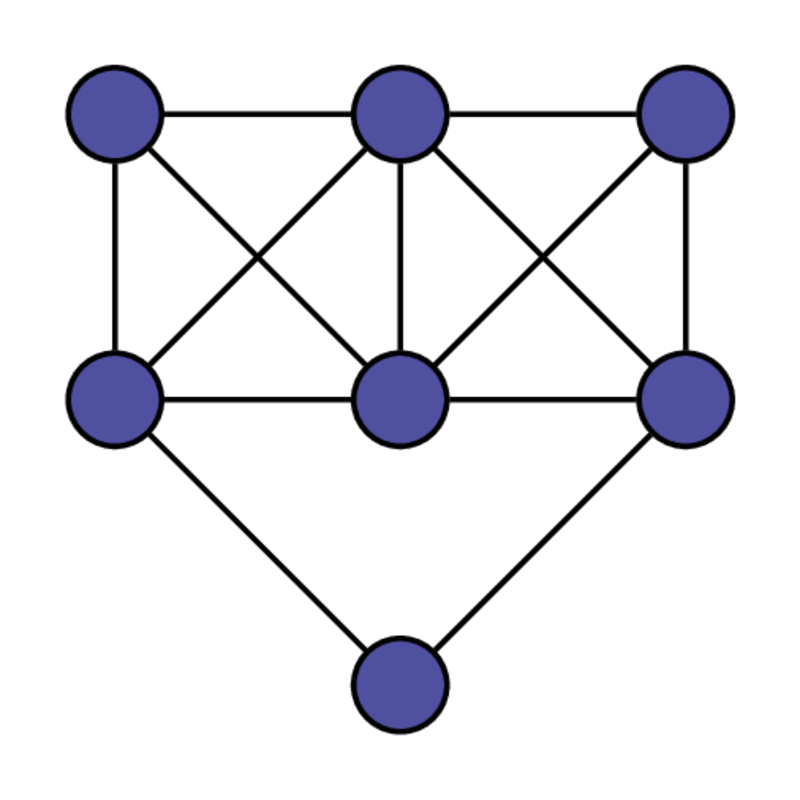
\includegraphics[width=.3\textwidth]{./exercise2/diagrams/d1.png} \end{center}
\item Ο αριθμός των ακμών είναι μεγαλύτερος απο 12 που είναι ο μέγιστος αριθμός ακμών που θα μπορούσε να έχει ένας διμερής γράφος με τους παραπάνω κόμβους και επομένως
      δεν είναι γραφική.
\item Μπορώ με χρήση επαγωγής να δείξω πως κάθε τέτοια ακολουθία είναι γραφική. Για $k=2$ έχουμε $(1,1)$ που προφανώς είναι γραφική ώς γράφος που αποτελείται
απο ένα ζεύγος. Έστω πως ισχύει για $k \ge 2$, τότε έχουμε $(k,k,k-1,k-1,...,1,1)$. Προσθέτω δύο κόμβους $v_{k+1}, v_{k+2}$ στο γράφο. Συνδέω τον
        $v_{k+2}$ με κάθε δεύτερο κόμβο συγκεκριμένου βαθμού και έχω $(k+1,k,k,k-1,k-1,...,2,2,1)$. Συνδέω τον $v_{k+1}$ με τον $v_{k+2}$ και έχω
        $(k+1,k+1,k,k,...,1,1)$ επομένως θα ισχύει και για $k+1$. Απο επαγωγή θα ισχύει και για όλα τα $k \ge 2$.

    
\end{enumerate}


